\chapter{Discussion of Experiences}

\section{New knowledge and skills gained in each of the duties and responsibilities}
\subsection{Duties and Responsibilities}
During the internship period, my field supervisor did not assign individual duties and responsibilities, but rather I was required to work with them as they did their daily tasks. My mandate was to have a positive attitude towards the training and show respect to my supervisor and other people we worked with. Therefore, my duty was to work willingly and adhere to tasks I was assigned to do. \\
The following are the main duties and responsibilities that I undertook during the field at BPW.\\
\textbf{End User Support:} I offered end user support on two systems of the company which included:
\begin{itemize}
\item[1.] \textbf{OCMS-BIM:} It is used in stock taking.
\item[2.] \textbf{Egatee:} It is used in e-sales.
\end{itemize}
\textbf{Digital Marketing:} I developed a messenger chatbot for the company as I was instructed by my supervisor which really worked well for BPW because it led to an increase in the sales and inquiries people were making through their facebook fanspage.\\ \\
\textbf{Software installations Installation:} I installed and configured software programs on both Linux and Windows platforms on the employees' computers at BPW.\\
\subsection{New knowledge and skills}
In the internship I accumulated a lot of knowledge and skills during the field attachment. Each of the duties and responsibilities as listed in section 3.1.1 empowered and greatly impacted on my career.\\
In each of the areas trained in, I was able acquire more skills and add on my experience like in installing softwares, anti­viruses, drivers, doing computer maintenance and repair I was able to work on numbers of computers, troubleshooting hardware and others.  
In the area of ethics and conduct, I was able to see and observe the working environment and how people behave and interact. I learnt a lot to do with interpersonal skills, good conduct and organizational culture. 

\section{Most interesting experiences}
During this Field Attachment period, I really enjoyed the experience of working at BPW
including  the  comfortable  working  atmosphere, the friendly relationship among the staff exhibited. Out of all these interesting moments, four extremely interesting experiences are highlighted below.
\subsection{Exhibition of the Infinix Note 5}
One of the very interesting experiences during this internship period was when 
Transsion Holdings officially unveiled the anticipated Infinix Note 5 at a media event held at the Hotel Triangle, in Kampala. The launch of the phablet follows the global launch that was held in Dubai over the weekend. \\
The Infinix Note 5 becomes the third (3rd) phablet Transsion Holdings under Infinix has launched this year. Following the success of the Infinix S3 and the Infinix Hot 6 and Hot 6 Pro which were launched in March and June respectively.

\begin{figure}[h!]
\begin{center}
	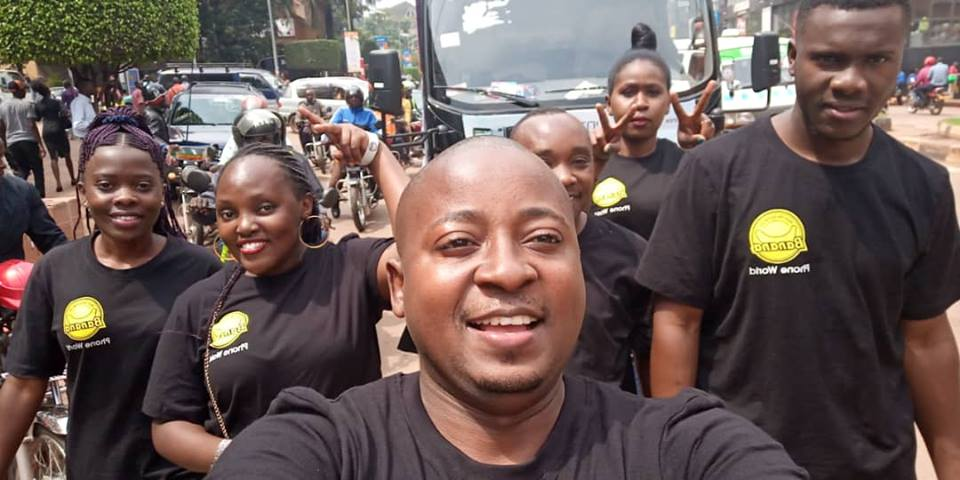
\includegraphics[scale=0.4]{img/klaus.jpg}
	\caption{Me at the extreme right during the exhibition.}
	\label{fig:symbols}
\end{center}
\end{figure}
\newpage
\subsection{Cloning of the Hard Disk}
\noindent Cloning of Hard Disk to install Windows and Ubuntu onto computers whereby
we installed everything at once without need to install application software,
everything was already installed, it was like copying the other Hard Disk onto
the computers.


\section{Relatedness of University's programmes to the Field of work}
Bachelor of Science in Computer Science program at Makerere University provides
professionals with theoretical and practical skills in the IT sector with the aim of
impacting knowledge and skills in fields such as networking, system Administration,
web designing and security management.\\ \\
During my two years I have studied quite a number of course units such as Computer
Literacy, Communication Skills and Operating System to mention but a few.All these course units are clearly related to duties I engaged in while at BPW and they are clearly explained in detail below.
\begin{itemize}
\item[*] Communication Skills was applied in effective speaking and listening skills that were taught at university  during  communications,  meetings  and  presentation sessions.
\item[*] Computer Literacy  skills  such as Microsoft Word, Excel and power point  to  prepare  professionally  looking  and  standard documents at work.
\item[*] Operating Systems was aplied in the windows and linux installation. 

\end{itemize}
These are just a few selected courses showing how the taught university programs are indeed relevant in the field of work. Even other courses not mentioned here, such as those in the field of networking are relevant, only that the intern never undertook tasks in that field during this period.
\section{Challanges faced and how managed}
Just like in any other organization, one is bound to experience a number of problems both at places of work and individual problems. The problems faced were related to work and these included the following.
\begin{itemize}
\item Time management challenged me in that I had to wake up very early to dodge the traffic jam so as I’m always early at my workplace. This proved to be a challenge to me but with time I coupled up with it.
\item I was challenged with the problem of money since this included transport and lunch. At times we were given some research work and this needed me to buy some internet bundles to inject in so as to buy data for my research work. I had my savings and my parents also provided me with some cash.
\item I was challenged with the problem of software incompatibility required to be installed onto the employees' computers. The software I always had required a 64 Bit computer and yet some machines were 32 bit machines.So I had to download some software from the internet which was compatible with those machines.
\end{itemize}
\section{Benefits derived from Field Attachment}
Besides the knowledge and skills talked about, the intership training gave me an opportunity to connect and interact with people in the same profession and people from different parts of the world.
\begin{itemize}
\item I gained a skill of time management and responsiveness of the duties and
activities assigned to me.
\item The training also enabled me to create useful friends who will motivate me in my carrier. I also got opportunity of being exposed to challenges at places of work and how they can be resolved.
\item I gained skills in online marketing and content management at large.
\item I learnt alot about smartphones especially Tecno, Infinix and Itel models.
\end{itemize} 
\section{Career Motivation}
While at BPW, I've been motivated to work harder, be creative and innovative in
different aspects as this would encourage me stay focused since most organizations
need creative IT persons.\\ \\
My internship attachment at BPW also helped me gain more professional skills that aren't gained in lecture rooms. This encouraged me to equip myself with all basic skills and enchance my CV in the future.
